\bchapter{Modello}
Il modello utilizzato nell'applicazione è una componente fondamentale per il rilevamento degli oggetti e si tratta di un modello di tipo Object Detection.
È importante sottolineare che questo modello è pre-allenato, il che significa che è stato precedentemente addestrato su un ampio set di dati per riconoscere
una vasta gamma di oggetti. Ciò consente all'applicazione di identificare oggetti in tempo reale attraverso la fotocamera del dispositivo.
Sebbene il modello fosse già disponibile come esempio in TFLite, abbiamo riscritto da zero il codice per adattarlo alle nostre esigenze specifiche e
garantire un'integrazione senza problemi con l'interfaccia utente dell'applicazione. Inoltre il codice fornito con l’esempio risultava ad oggi obsoleto.

L'interfaccia fornita dal modello è progettata per essere intuitiva e semplice da utilizzare. L'unico tipo di input supportato è un'immagine Bitmap con
dimensioni di 300 x 300 pixel e tre canali per pixel (RGB). È importante notare che i valori dei pixel nell'immagine sono di tipo uint8, ovvero valori
senza segno su 8 bit che variano da 0 a 255.
Tuttavia, le fotocamere dei dispositivi moderni possono raggiungere risoluzioni molto più elevate, come il formato 4K (3840 x 2160) o almeno in HD. Di
conseguenza, abbiamo dovuto implementare una logica per convertire l'immagine catturata dalla fotocamera in un formato compatibile con le dimensioni di
input richieste dal modello, cioè 300 x 300 pixel.

Una delle caratteristiche chiave del modello è la possibilità di selezionare il delegato da utilizzare per l'esecuzione delle inferenze. Di default, il
delegato utilizzato è il processore (CPU), ma è possibile cambiare questa impostazione tramite una finestra a tendina nell'interfaccia utente
dell'applicazione. I delegati disponibili includono CPU, GPU e NNAPI (Android Neural Networks API), che offrono prestazioni e ottimizzazioni specifiche
per il dispositivo in uso.
È importante sottolineare che l'applicazione è progettata per gestire eventuali errori o incompatibilità durante l'utilizzo dei diversi delegati per
l'esecuzione del modello. Se il delegato selezionato non è supportato sul dispositivo in uso, verrà visualizzato un messaggio di errore, ma l'applicazione
continuerà a funzionare senza interruzioni. Questo garantisce un'esperienza utente fluida e affidabile anche in condizioni non ideali.

Inoltre, nell'interfaccia utente della fotocamera, è presente un overlay fisso che mostra i risultati del rilevamento degli oggetti. Questi risultati sono
rappresentati da rettangoli posizionati sull'immagine in base alla posizione degli oggetti rilevati. Ogni rettangolo è accompagnato da informazioni sulla
categoria dell'oggetto e il punteggio di confidenza associato.

Per garantire una visualizzazione accurata dei risultati, è necessario applicare un fattore di scala per adattare le coordinate dei rettangoli dalla
dimensione della bitmap utilizzata dal modello alla dimensione effettiva dell'immagine catturata dalla fotocamera. Questo processo assicura che i rettangoli
siano correttamente sovrapposti all'oggetto rilevato nell'immagine visualizzata e che non siano presenti rettangoli che fuoriescono dai bordi imposti dallo
schermo, in modo da renderli sempre totalmente leggibili.

Inoltre, l'applicazione offre la possibilità di personalizzare la soglia di confidenza per il rilevamento degli oggetti e il numero massimo di risultati da
visualizzare contemporaneamente. Anche queste impostazioni possono essere regolate dall'utente tramite la finestra a tendina nell'interfaccia utente e
vengono salvate per essere applicate automaticamente ad ogni avvio dell'applicazione.
Ogni modifica viene salvata in una SharedPreference che permette il salvataggio e il ripristino delle scelte ad ogni avvio dell’app.

Per garantire una forte user experience è stato adottato un controllo sui risultati presenti. In particolare, se i risultati ottenuti non cambiano, ovvero
rimangono intatti come numero e come classi ottenute, allora la visualizzazione viene modificata solo ogni secondo. Nel momento in cui è presente una classe
in più o in meno o ci sono differenze, viene aggiornata la visione. Questo permette di non vedere troppe informazioni in continua modifica a schermo. Il
tutto è realizzato tramite l’utilizzo di un timer non bloccante e un semplice controllo in retroazione.

In figura \ref{fig:modello} si può vedere l’immagine che descrive I/O del modello.

\begin{figure}[ht]
    \centering
    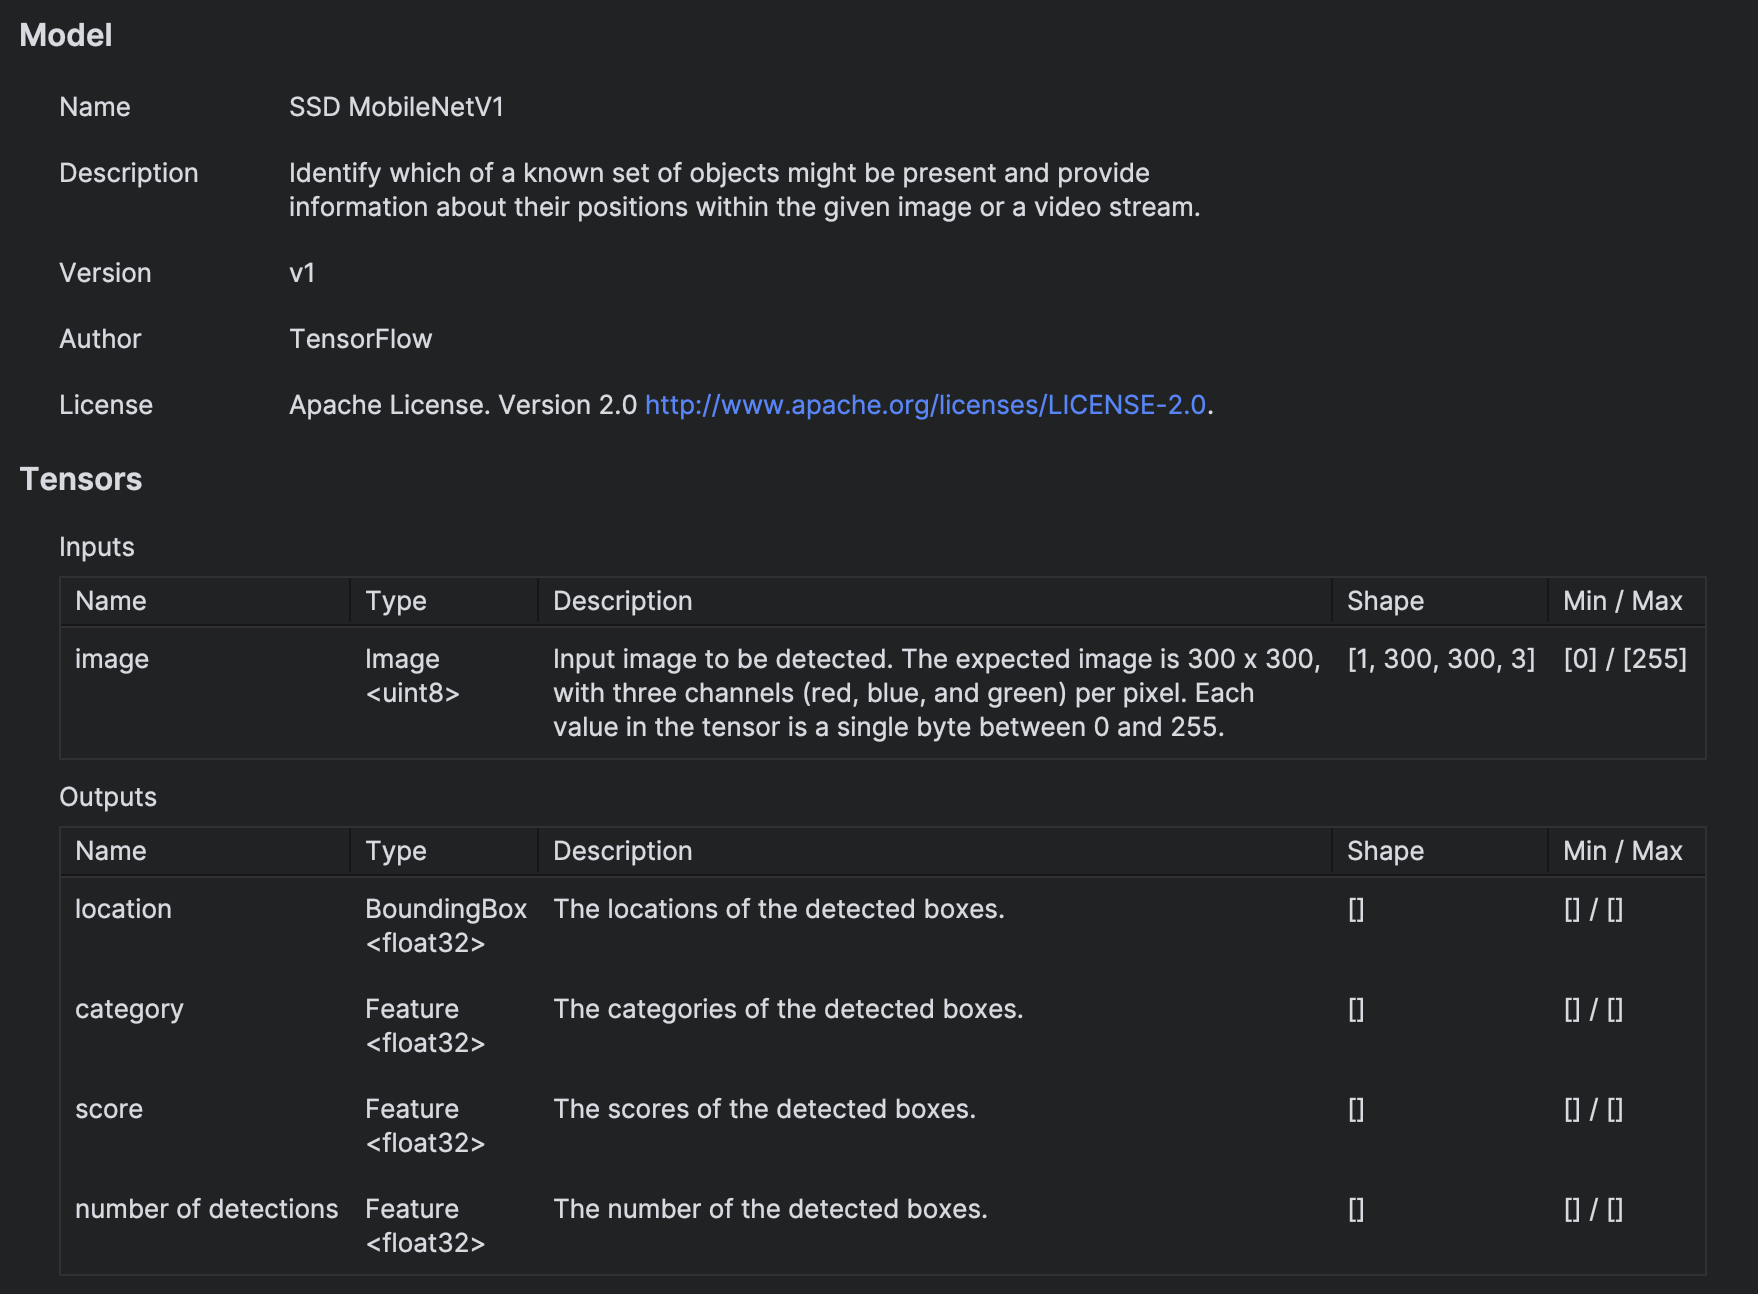
\includegraphics[width=0.8\textwidth]{Immagini/App/modello.png}
    \caption{I/O del modello}
    \label{fig:modello}
\end{figure}
